\chapter{Port Knocking}

Le Port Knocking est un des modèles qui a été inventé pour répondre au besoin d'ouverture et de fermeture automatique de ports.

Dans ce modèle, la client s'authentifie auprès du serveur en lançant des tentatives de connexions (à l'aide de paquets SYN) sur certains ports spécifiques constituant un code. Le serveur ouvre un port seulement si le même émetteur réalise la bonne séquence de tentative de connexion.

Cette solution nécessite peu de ressource et est aisée à mettre en place, cependant une simple écoute du réseau permet de repérer le code permettant l'ouverture d'un port ce qui rend cette solution facilement attaquable.

Par exemple, si la séquence de port à fournir au pare-feu afin de rendre le port \emph{E} du serveur joignable est [\emph{Port A, Port B, Port C, Port D}] , le client génère des paquets SYN sur ces ports dans l'ordre donné:
\begin{figure}[h]

\centerline{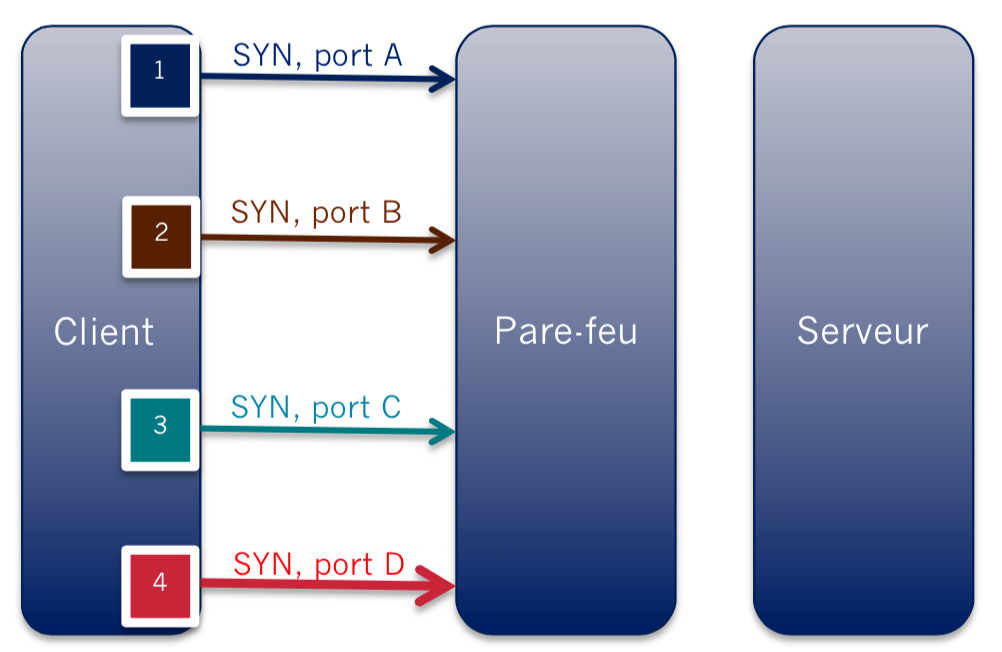
\includegraphics[scale=0.4]{portknocking1}}

\end{figure}

Après avoir vérifier la validité de la séquence, le pare-feu accorde au client l'accès au port \emph{E} : 

\begin{figure}[h]

\centerline{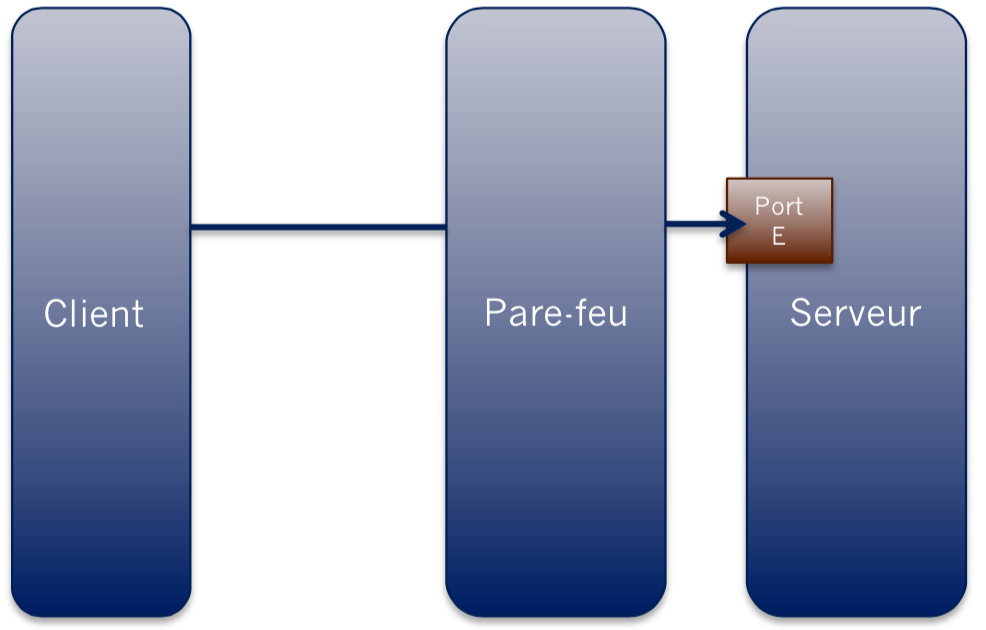
\includegraphics[scale=0.4]{portknocking2}}

\end{figure}